\pdfcompresslevel=0
\documentclass[a0paper, portrait]{tikzposter} % See Section 3
\tikzposterlatexaffectionproofoff

%\usepackage[cmyk]{xcolor}
\definecolor{UPCblue}{cmyk}{1,0.34,0,0.02}
\usepackage{pgfplots}
\pgfplotsset{compat=1.8}

\usepackage{svg}
\usepackage{qrcode}
\usepackage{adjustbox}
\usepackage{booktabs}
\usepackage{caption}

\usepackage{lmodern}

\title{\parbox{\linewidth}{\centering \DPmst: a concurrent algorithm to maintain dynamically minimum spanning trees}}
\institute{Universitat Politècnica de Catalunya} % See Section 4.1
\author{D. Benedí$^*$, A. Duch, E. Pasarella, C. Zoltan}
\titlegraphic{
\includegraphics[]{upc_white.png}}


%\usetheme{Default} % See Section 5
\definecolorpalette{ColorPalette} {
    \definecolor{colorOne}{named}{white}
    \definecolor{colorTwo}{named}{black}
    \definecolor{colorThree}{named}{UPCblue}
}
\definecolorstyle{ColorStyle} {
    \definecolor{colorOne}{named}{white}
    \definecolor{colorTwo}{named}{black}
    \definecolor{colorThree}{named}{UPCblue}
}{
    % Background Colors
    \colorlet{backgroundcolor}{colorOne}
    \colorlet{framecolor}{black}
    % Title Colors
    \colorlet{titlefgcolor}{colorOne}
    \colorlet{titlebgcolor}{colorThree}
    \colorlet{titlecolor}{colorTwo}
    % Block Colors
    \colorlet{blocktitlebgcolor}{colorThree}
    \colorlet{blocktitlefgcolor}{black}
    \colorlet{blockbodybgcolor}{white}
    \colorlet{blockbodyfgcolor}{black}
    % Innerblock Colors
    \colorlet{innerblocktitlebgcolor}{white}
    \colorlet{innerblocktitlefgcolor}{black}
    \colorlet{innerblockbodybgcolor}{colorThree!30!white}
    \colorlet{innerblockbodyfgcolor}{black}
    % Note colors
    \colorlet{notefgcolor}{black}
    \colorlet{notebgcolor}{yellow!50!white}
    \colorlet{noteframecolor}{colorTwo} % I don't know
}
\usecolorstyle[colorPalette=ColorPalette]{ColorStyle}

\definebackgroundstyle{BackgroundStyle}{
    \draw[inner sep=0pt, line width=0pt, color=backgroundcolor, fill=backgroundcolor]
    (bottomleft) rectangle (topright);
}
\usebackgroundstyle{BackgroundStyle}

\definetitlestyle{TitleStyle}{
    width=\paperwidth, linewidth=0pt, innersep=5pt,
    titletotopverticalspace=0mm, titletoblockverticalspace=40mm
}{
    \begin{scope}[line width=\titlelinewidth]
        % Background
        \fill[UPCblue]
        (\titleposleft, \titlepostop) -- % Top left corner
        (\titleposright, \titlepostop) -- % Top right corner
        (\titleposright, \titleposbottom - 2cm) % Bottom right corner
        .. controls ({(\titleposright + \titleposleft) / 2}, \titleposbottom+0cm) .. % Pass by point
        (\titleposleft, \titleposbottom - 2cm) -- % Bottom left corner
        cycle;
        % Underline
        \draw[UPCblue, line width=10pt] 
        (\titleposright, \titleposbottom - 2.5cm) .. controls
        ({(\titleposright + \titleposleft) / 2}, \titleposbottom-0.5cm) ..
        (\titleposleft, \titleposbottom - 2.5cm);
        % Logo UPC
        \node[] (logo) at ( \titleposright - 11cm , \titleposbottom + 3cm) {
\includegraphics[]{upc_white.png}};
        % Logo EuroPar
        \node[] (logo) at ( \titleposleft + 11cm , \titleposbottom + 3cm) {\includesvg[width=17cm]{Euro-Par-2024-logo_sp.svg}};
    \end{scope}
}
\usetitlestyle{TitleStyle}

\defineblockstyle{BlockStyle} {
    titlewidthscale=0.9, bodywidthscale=1, titlecenter,
    titleoffsetx=0pt, titleoffsety=0pt, bodyoffsetx=0mm, bodyoffsety=15mm,
    bodyverticalshift=10mm, roundedcorners=0, linewidth=0pt,
    titleinnersep=6mm, bodyinnersep=1cm
} {
    \ifBlockHasTitle
    %\draw[UPCblue, line width=5pt, dashed] ({(blockbody.north west + blocktitle.south west) / 2}) to ({(blockbody.north east + blocktitle.south east) / 2});
        \draw[black!50!white, loosely dotted, ultra thick] (blocktitle.south west) to (blocktitle.south east);
    \fi
}
\useblockstyle{BlockStyle}

\makeatletter
\settitle{ 
  \centering
  \begin{minipage}[t]{0.7\textwidth}
    \centering
    \vspace*{2em}
    \color{white}
    {\bfseries \Huge \sc \textbf{ \@title } \par}
    \vspace*{1em}
    {\huge \textbf{ \@author } \par}
    \vspace*{1em}
    {\Large \textbf{ \@institute }}
    \vspace*{0.5em}\\
    {\large \textbf{ $^*$Contact: daniel.benedi@upc.edu }}
    \vspace*{0.5em}    
  \end{minipage}%
}
\makeatother

\usepackage{tikz}
\usetikzlibrary{positioning,quotes,shapes.geometric,arrows.meta}
\pgfdeclarelayer{nodelayer} 
\pgfdeclarelayer{edgelayer}
\pgfdeclarelayer{embeded}
\pgfdeclarelayer{stages}
\pgfsetlayers{backgroundlayer,main,notelayer,nodelayer,edgelayer,embeded,stages}
\tikzstyle{new style 0}=[fill=white, line width=1mm, draw=black, shape=circle, align=center,minimum size=2cm,scale=1.75]
\tikzstyle{tree_edge}=[-, line width=1mm, draw=black,font=\LARGE]
\tikzstyle{opChan}=[-{Stealth[length=6mm]}, black, line width=1mm]
\tikzstyle{daChan}=[-{Stealth[length=6mm]}, red, line width=1mm]
\tikzstyle{io}=[trapezium, trapezium angle=67, trapezium stretches body, fill=blue!30, draw=black,  line width=1mm,]
\tikzstyle {filter_gen} = [rectangle, rounded corners, text centered, draw=black, fill=UPCblue!30,  line width=1mm,]

\newcommand{\instancename}{DP-Instance}
\newcounter{instance}

\newcommand{\mst}{$\mathsf{MST}$}
\newcommand{\msts}{$\mathsf{MST}$s}
\newcommand{\mstof}[1]{$\mathsf{MST}_{#1}$}
\newcommand{\dynmst}{\mathsf{Dynamic\_MST}}
\newcommand{\dpm}{$\mathsf{DPM}$}
\newcommand{\DP}{$\mathsf{DP}$}
\newcommand{\DPmst}{\texttt{DP\_{Kruskal}}}
\newcommand{\DPmstv}[1]{\texttt{DP\_{{#1}}}}
\newcommand{\FKruskal}{\texttt{Filter\_{Kruskal}}}
\newcommand{\Kruskal}{\texttt{Kruskal}}

\newcommand{\Go}{{\tt Go}}
\newcommand{\Golang}{{\tt Golang}}


\begin{document}
\maketitle % See Section 4.1

\begin{columns}
  \column{0.5}
    \block{Introduction}{
        We {\bf introduce} \DPmst: a parallel and concurrent Kruskal-based algorithm,  {\bf defined} on the Dynamic Pipeline Model (\dpm)~\cite{Pasarella2024}, to {\bf solve} the fundamental Minimum Spanning Tree (\mst) problem.
        \DPmst\ {\bf outperforms} other algorithms and is particularly {\bf effective} for {\bf dense} graphs.
        
        %Various parallelization methods have been explored to enhance the efficiency of sequential \mst\ algorithms, resulting in multiple parallel algorithms~\cite{durbhakula2020parallel}.
    }
    
    \column{0.5}
    \block{\DPmst}{
        A \emph{dynamic pipeline} (DP) is a sequence of {\bf connected} (via communication channels) \textbf{concurrent, stateful stages}. \DPmst\ distributes the input graph $G=(V,E)$ along a DP with event and graph channels carrying events and \msts, respectively. 
    }
\end{columns}

% Middle DP Figure
\begin{columns}
    \column{0.17}
    \block[bodyverticalshift=-30mm,bodyoffsety=-35mm]{}{
    \begin{tikzpicture}
        \begin{pgfonlayer}{nodelayer}
            \node[style=new style 0, scale=0.8] (a) at (0,0) {a};
            \node[style=new style 0, scale=0.8, above=3cm of a] (b) {b};
            \node[style=new style 0, scale=0.8, below right=3.2cm of a] (c) {c};
            \node[style=new style 0, scale=0.8, below left=3.2cm of a] (d) {d};
            \node[style=new style 0, scale=0.8, below=3cm of c] (e) {e};
            \node[style=new style 0, scale=0.8, below=3cm of d] (f) {f};
        \end{pgfonlayer}
        \begin{pgfonlayer}{edgelayer}
            \draw[style={tree_edge}]{} (b) to["0.4"] (a);
            \draw[style={tree_edge}]{} (c) to["0.3"] (d);
            \draw[style={tree_edge}]{} (a) to["0.6"] (c);
            \draw[style={tree_edge}]{} (d) to["0.1"] (f);
            \draw[style={tree_edge}]{} (d) to["0.8"] (a);
            \draw[style={tree_edge}]{} (c) to["0.9"] (e);
        \end{pgfonlayer}
    \end{tikzpicture}
    }  
    \column{0.65}
    \block[bodyverticalshift=-30mm,bodyoffsety=-35mm]{}{
    \begin{tikzpicture}
        \begin{pgfonlayer}{nodelayer}
            \node (ref) at (0,0) {};
            \node [style=io, minimum height=3.59cm, minimum width=14.56cm, shape border rotate=270,fill=red!30, below=1.727cm of ref] (In) {\huge I};
            \node [style=filter_gen, minimum width=6.72cm, minimum height=11.2cm, right= 3.36cm of In,  text depth = 6.72cm] (F1) {\huge $F_a$};
            \node [style=filter_gen, minimum width=6.72cm, minimum height=11.2cm, right= 3.36cm of F1,  text depth = 6.72cm] (F2) {\huge $F_c$};
            \node [style=filter_gen, minimum width=6.72cm, minimum height=11.2cm, right= 3.36cm of F2,  text depth = 6.72cm] (F3) {\huge $F_d$};
            \node [style=filter_gen, minimum width=6.72cm, minimum height=11.2cm, align=center, right= 3.36cm of F3, fill=green!30] (Gen) {\huge Gen};
            \node [style=io, minimum height=3.59cm, minimum width=14.56cm, shape border rotate=90, right= 3.36cm of Gen, fill=gray!30] (Out) {\huge O};
        \end{pgfonlayer}
        
        \begin{pgfonlayer}{edgelayer}
                \draw [style={opChan}] ([yshift=2.24 cm]Gen.east) to["Op"] ([yshift=2.24 cm]Out.west);
                \draw [style={daChan}] ([yshift=-2.24 cm]Gen.east) to["\mst\ "] ([yshift=-2.24 cm]Out.west);

                \draw [style={opChan}] ([yshift=2.24 cm]In.east) to["Op"] ([yshift=2.24 cm]F1.west);
                \draw [style={daChan}] ([yshift=-2.24 cm]In.east) to["\mst\ "] ([yshift=-2.24 cm]F1.west);
                
                \draw [style={opChan}] ([yshift=2.24 cm]F1.east) to["Op"] ([yshift=2.24 cm]F2.west);
                \draw [style={daChan}] ([yshift=-2.24 cm]F1.east) to["\mst\ "] ([yshift=-2.24 cm]F2.west);
                
                \draw [style={opChan}] ([yshift=2.24 cm]F2.east) to["Op"] ([yshift=2.24 cm]F3.west);
                \draw [style={daChan}] ([yshift=-2.24 cm]F2.east) to["\mst\ "] ([yshift=-2.24 cm]F3.west);
                \draw [style={opChan}] ([yshift=2.24 cm]F3.east) to["Op"] ([yshift=2.24 cm]Gen.west);
                \draw [style={daChan}] ([yshift=-2.24 cm]F3.east) to["\mst\ "] ([yshift=-2.24 cm]Gen.west);
        \end{pgfonlayer}

        \begin{pgfonlayer}{embeded}
            %Filter 1
            \node [style=new style 0, scale=0.56] (a1) at (F1) {a};
            \node [style=new style 0, scale=0.56,below=0.81cm of a1] (b1) {b};
            \node [style=new style 0, scale=0.56,below left=1.23cm of a1] (c1) {c};
            \node [style=new style 0, scale=0.56,below right=1.23cm of a1] (d1) {d};
            \draw[style={tree_edge}]{} (a1) to (b1);
            \draw[style={tree_edge}]{} (a1) to (c1);
            \draw[style={tree_edge}]{} (a1) to (d1);
            
            %Filter 2
            \node [style=new style 0, scale=0.56] (c2) at (F2) {c};
            \node [style=new style 0, scale=0.56,below left=1.23cm of c2] (d2) {d};
            \node [style=new style 0, scale=0.56,below right=1.23cm of c2] (e2) {e};
            \draw[style={tree_edge}]{} (c2) to (d2);
            \draw[style={tree_edge}]{} (c2) to (e2);
            
            %Filter 3
            \node [style=new style 0, scale=0.56] (d3) at (F3) {d};
            \node [style=new style 0, scale=0.56,below=0.81cm of d3] (f3) {f};
            \draw[style={tree_edge}]{} (d3) to (f3);
        \end{pgfonlayer}
        
    \end{tikzpicture}
     \captionof{figure}{\label{fig:dp_example}An instance of \DPmst}  
    }
    \column{0.17}
    \block[bodyverticalshift=-30mm,bodyoffsety=-35mm]{}{
    \begin{tikzpicture}
        \begin{pgfonlayer}{nodelayer}
            \node[style=new style 0, scale=0.8] (a) at (0,0) {a};
            \node[style=new style 0, scale=0.8, above=3cm of a] (b) {b};
            \node[style=new style 0, scale=0.8, below right=3.2cm of a] (c) {c};
            \node[style=new style 0, scale=0.8, below left=3.2cm of a] (d) {d};
            \node[style=new style 0, scale=0.8, below=3cm of c] (e) {e};
            \node[style=new style 0, scale=0.8, below=3cm of d] (f) {f};
        \end{pgfonlayer}
        \begin{pgfonlayer}{edgelayer}
            \draw[style={tree_edge}]{} (b) to["0.4"] (a);
            \draw[style={tree_edge}]{} (c) to["0.3"] (d);
            \draw[style={tree_edge}]{} (a) to["0.6"] (c);
            \draw[style={tree_edge}]{} (d) to["0.1"] (f);
            \draw[style={tree_edge}]{} (c) to["0.9"] (e);
        \end{pgfonlayer}
    \end{tikzpicture}
    }
\end{columns}

\block{Instance of \DPmst}{
Figure \ref{fig:dp_example} illustrates an instance of \DPmst. It consists of:
        \begin{itemize}
          \item \emph{Input ($I$):} Receives events of the form $({\tt op, e})$ and passes them through the event channel; if ${\tt op} = {\tt mst}$, sends an empty set via the graph channel.
           \item \emph{Filter ($F_v$):} $v$ is a vertex, called the \emph{root} of the filter. When an event $({\tt op,e})$ arrives: 
                (i) If ${\tt op} \in \{{\tt insert, update, delete}\}$ and $e$ is incident to $v$, processes the event; otherwise, passes it to the next stage. 
                (ii) If ${\tt op} = {\tt mst}$, computes a partial \mst\ from the union of the arriving \mst\ and the tree in $F(v)$, then passes it to the next stage.
            \item \emph{Generator ($Gen$):} If ${\tt op} \in \{{\tt insert, update}\}$ arrives, spawns a new Filter stage $F(v)$, adding it to the pipeline between the last filter and $Gen$.
            \item \emph{Output ($O$):} If ${\tt op} = {\tt mst}$ arrives, outputs the \mstof{G}.
        \end{itemize}
    }



\block[titleoffsety=25mm,bodyoffsety=40mm]{Single core and Static random graphs}{
      \begin{adjustbox}{valign=t}
      \begin{minipage}[t]{0.63\linewidth}
            \centering
            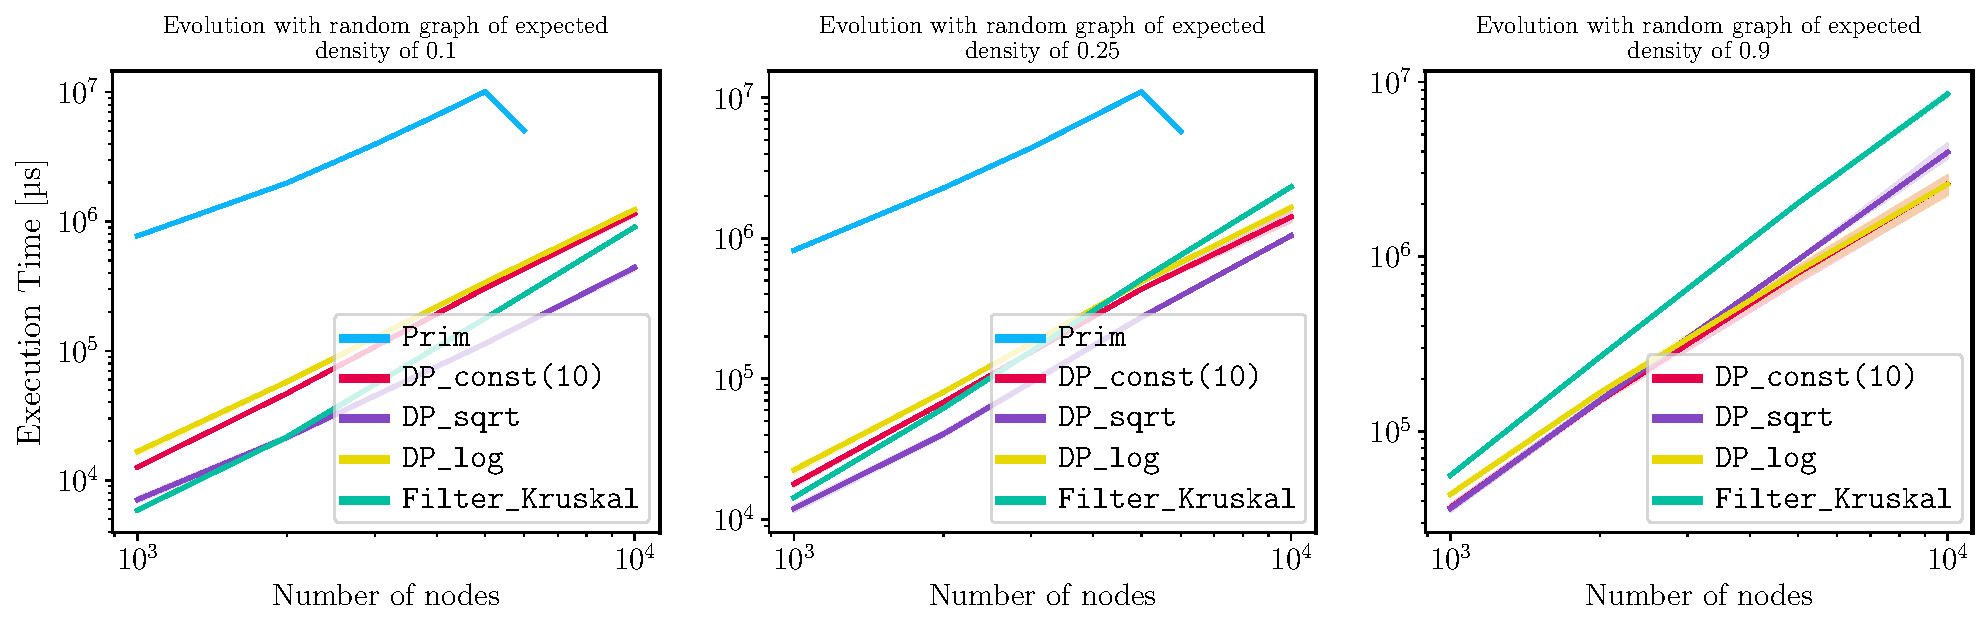
\includegraphics[width=\linewidth]{figs/SomeDensities_mixed.pdf}
            \captionof{figure}{\label{fig:dpmst-versions}Comparison of \DPmst\ with different root numbers per filter: \DPmstv{const(10)}, \DPmstv{log}, and \DPmstv{sqrt}; and with other algorithms on a single core over random graphs of $n$ vertices. For each size and probability 20 random graphs were generated }
      \end{minipage}%
      \end{adjustbox}
      %
      \hspace{1cm}
      \begin{minipage}[t]{0.35\linewidth}
      
       \vspace{1cm}
       
      We compared \DPmst\ against (i) \FKruskal~\cite{Osipov2009}, and (ii) a message-passing {\tt Prim}~\cite{Loncar2014} implementation on a single core and randomly generated graphs of $n$ vertices studying the {\bf effect of the number of roots} in each filter of \DPmst\; three options were considered: (a) a constant number of roots \DPmstv{const},  (b) $\log(n)$ roots \DPmstv{log}, and (c) $\sqrt{n}$ roots \DPmstv{sqrt}. 
      
      \vspace{1cm}
      
      Although for small graphs, \FKruskal\ is faster; as \textbf{graph size and density increase}, \DPmstv{sqrt}\ becomes the \textbf{best option} (see Figure \ref{fig:dpmst-versions}).
      \end{minipage} 
}

\block[titleoffsety=15mm,bodyoffsety=30mm]{Multi core and Dynamic real graphs}{
      \begin{minipage}[t]{0.35\linewidth} 
        We compare \DPmst\ and \FKruskal\ on realistic dynamic graphs obtained from DynGraphLab~\cite{HanHenSchuSurvey2021}. We observe that:
        \begin{itemize}
            \item \DPmst\ is effective for maintaining the \mst\ (See Table \ref{tab:real_graphs_time}).
            \item  \DPmst\ has \textbf{excellent performance} in a parallel environment, showcasing \textbf{significant scalability} (See Figure \ref{fig:real_graphs_speed}).
        \end{itemize}
      \vspace{1cm}
       \begin{center}
            \resizebox{0.8\textwidth}{!}{%
            \begin{tabular}{lcccc}
                \toprule
                Dataset & $n$ & op. & \FKruskal & \DPmst\ \\
                \midrule
                {\tt as-caida}     &31379 &119468&  1h 30min &  1h 19min \\
                {\tt movielens10m} &49847&384585&  1h 39min &  1h 20min \\
                {\tt simplewiki}   &100312&889016 &17h  8min & 11h 29min \\
                \bottomrule
            \end{tabular}
            }\\
            \captionof{table}{\label{tab:real_graphs_time}Time with 1 core and 10 roots per filter}
        \end{center}
      \end{minipage}%
      %
      \hspace{1cm}
      \begin{adjustbox}{valign=t}
      \begin{minipage}[t]{0.63\linewidth}
            \centering
            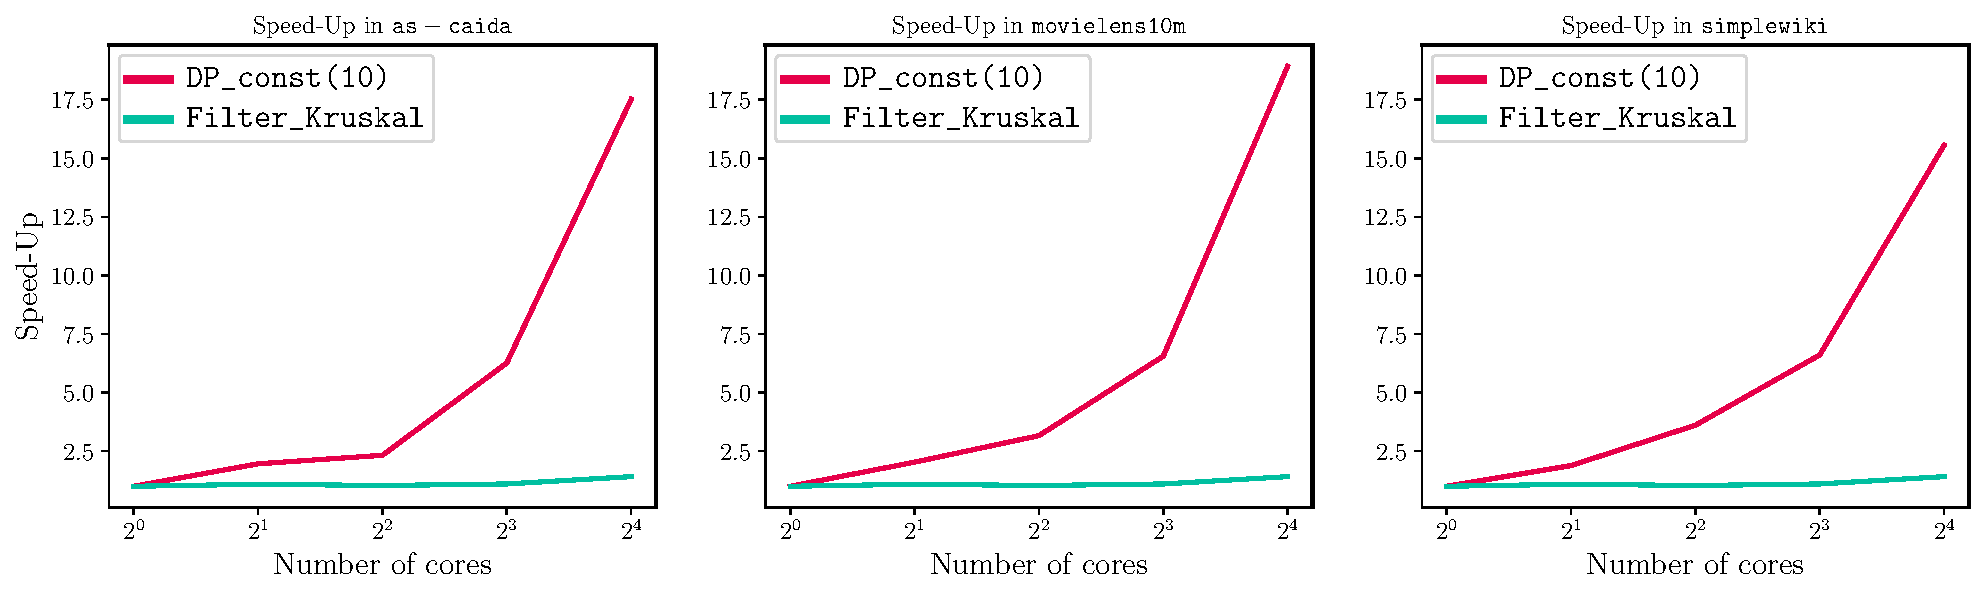
\includegraphics[width=1\linewidth]{figs/RealGraphs.pdf}
            \captionof{figure}{\label{fig:real_graphs_speed}Multicore comparison of speed-ups}
      \end{minipage} 
      \end{adjustbox}
}

\begin{columns}
    \column{0.45}
    \block[titleoffsety=15mm,bodyoffsety=30mm]{Final Remarks}{
    \label{sec:ongoing}
    %We propose the \DPmst\ algorithm and we implemented it in \Go\ for its efficient handling of dynamic pipelines. 
    %We propose the \DPmst\ algorithm. 
    Experiments on random and real graphs demonstrate that the \DPmst\ algorithm is particularly \textbf{competitive for dense graphs}, showing improved performance over the \FKruskal\ algorithm for graphs with over $2 \cdot 10^3$ vertices. It also \textbf{scales well}, enhancing efficiency and speed up to 16 cores. 
    
    Future work includes for instance to compare \DPmst\ against a {\tt MapReduce}-based competitor~\cite{nowicki2021dynamic}; to evaluate other \mst\ algorithms within the \DPmst\ model; to assess different implementation languages; to experiment with larger datasets and other dynamic graph models.}
    \column{0.5}
    \block[titleoffsety=15mm,bodyoffsety=30mm]{References}{
        \begingroup
            \renewcommand{\section}[2]{}%
            \bibliographystyle{splncs04}
            \bibliography{short_biblio}
        \endgroup
    }
\end{columns}

\begin{scope}
    \node[color=black, align=center] (url) at (-8,-55.2) {\qrcode[version=1,height=4cm]{https://github.com/danielbenedi6/MasterThesis} };
    \node[color=black, align=center, below=2mm of url] (text) {Source Code};
\end{scope}

\end{document}